\section{Design Details}
The reference model for this project is shown in figure \ref{figure:refproblem}. 
The reference design is a paper impregnated with oil bushing with 21 aluminium foils of $100\mu m$.
One side of the bushing is exposed to air, the other to oil, similar to a transformer bushing.
The diameter of the conductor is 100mm, the bushing diameter is 300mm.
The length of the first foil is 5000mm long, and fixed 2mm into the bushing at the conductor voltage.
The outer foil is also set 2mm inside the bushing and is directly connected to the earthed flange.
The conductor is used at 275kV AC voltage, and the design was taken from a bushing that was in operation for around 30 years.
\begin{figure}[!h]
   \centering
   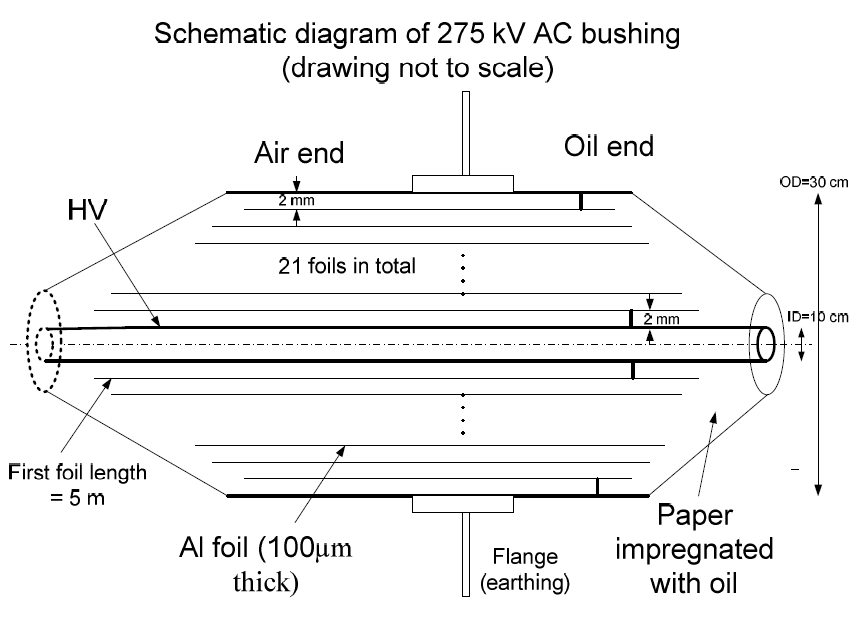
\includegraphics[width = 0.7\textwidth]{ReferenceDiagram.png}
   \caption{The reference problem taken from \cite{Chen14}}
   \label{figure:refproblem}
\end{figure}

\subsection{Design Issues}
In section \ref{ss:CapacitiveGrading} the initial information required for both radial and axial grading includes the length and radial displacement of the innermost foil.
In the reference design the following initial information is given.

\begin{table}[!htb]
\caption{Initial Information for Reference Design}
\label{table:initinfo}
\begin{center}
\begin{tabular}{cc}
\toprule
\textbf{Initial Information} & \textbf{Value)} \\ \toprule
Conductor Diameter (ID) & $100mm$ \\
First Foil Length $L_1$ & $5000mm$ \\
First Foil Radius $r_1$&$52mm$ \\
Outer Bushing Diameter (OD) & $300mm$\\
Outer Foil Radius $r_21$ & $148mm$\\
\bottomrule
\end{tabular}
\end{center}
\end{table} 

This information intuitively fits radial grading best, since there is no requirement to assume the length of the outermost foil.
However, there is a discrepancy between the standard literature problem and the reference design.
The first foil is connected to the high voltage conductor, and the last foil is connected to the earthed flange.
This is to eliminate the electric field on the boundary interface as far as possible on both sides of the bushing, so that the voltage drop occurs exclusively inside the bushing insulation.

This has an impact on the calculations described in section \ref{ss:CapacitiveGrading}.
Since the innermost foil is at the same voltage as the conductor, there is no capacitance between them, hence the first foil shown on the diagram is not the first index for the iterative calculation.
The derivation of the iterative equation assumes a capacitance between each foil. 
The first foil in figure \ref{figure:refproblem} is therefore indexed as zero.

This means that there is not sufficient initial information to proceed, since the first non-connected foil length $L_1$ is not given.
The iterative equations require the first non-connected foil length $L_1$ to be known as shown in equation \ref{eq:ref0}. 
All radii variables are known due to the even spacings under radial grading. 

\begin{equation}
   \label{eq:ref0}
   \displaystyle\frac{L_{1}}{ln(\displaystyle\frac{r_{1}}{r_{0}})} = \displaystyle\frac{ L_{2}}{ln(\displaystyle\frac{r_{2}}{r_{1}})} 
\end{equation}
\begin{equation}
   \label{eq:ref0forl1}
   L_{2} = L_{1}\displaystyle\frac{{ln(\displaystyle\frac{r_{2}}{r_{1}})} }{ln(\displaystyle\frac{r_{1}}{r_{0}})} 
\end{equation}

\inote{Insert figure with close up showing foil 0, 1 and 2 with 0 the closest to the conductor}

If this is not taken into account then a flawed design will be produced.
Equation \ref{eq:ref0wrongfilled} shows a wrongly described first iteration of the radial grading formula which results in the design in figure \ref{figure:flawedgraph}. This is clearly wrong, and does not give the hyperbolic shape from the beginning of the foils.
\begin{equation}
   \label{eq:ref0wrongfilled}
   L_{1} = 5000mm\displaystyle\frac{{ln(\displaystyle\frac{56.8mm}{52mm})} }{ln(\displaystyle\frac{52mm}{50mm})}
   = 11256mm
\end{equation}

\begin{figure}[!h]
   \centering
   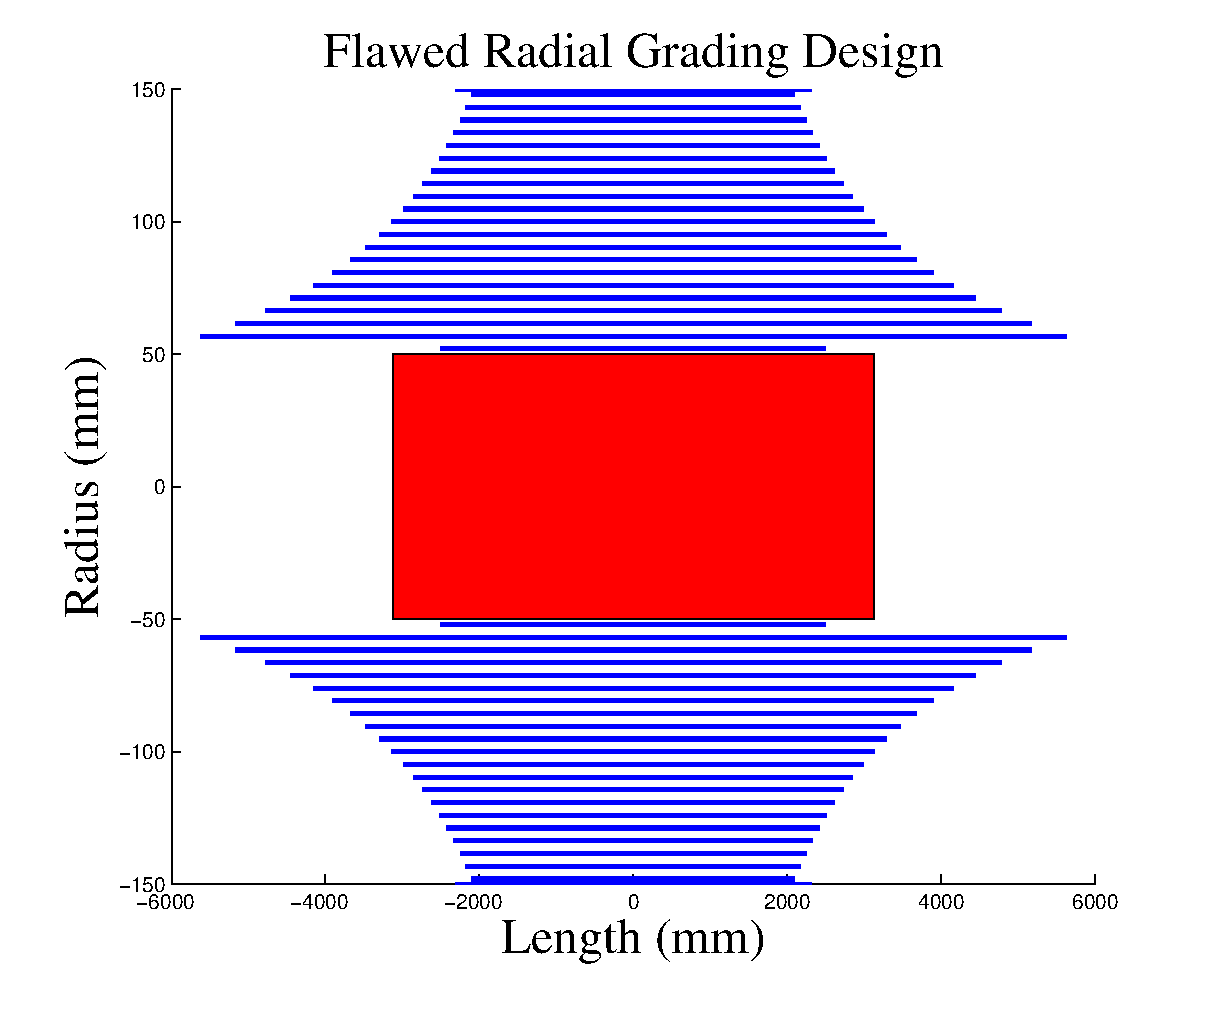
\includegraphics[width = 0.7\textwidth]{FlawedRadGradGraph.eps}
   \caption{Flawed Radial Grading Design}
   \label{figure:flawedgraph}
\end{figure}

In order to proceed with the calculations there must be an assumption of the length of the first unconnected foil.
A reasonable assumption is that this follows the hyperbolic shape of the other foils, which helps to evenly distribute the electric field.
To achieve this design mathematically, two assumptions are made.
\begin{enumerate}
\item Foil 0 is not connected to the HV conductor.
\item The conductor surface is spaced a distance of $S_n$ from foil 0.
\end{enumerate}
Assumption 1 is required to be able to use the capacitor derived iterative formula on foil 0.
Assumption 2 is required so that the radial spacing is kept constant.
The first iteration has been calculated under these assumptions, giving the result in equation \ref{eq:ref0correct} which is an expected value.
The remainder the foil parameters can then be calculated using the iterative formula.
\begin{equation}
   \label{eq:ref0correct}
   L_{1}
   = 5000mm\displaystyle\frac{{ln(\displaystyle\frac{56.8mm}{52mm})} }{ln(\displaystyle\frac{52mm}{47.2mm})}
   = 4558mm
\end{equation}

\subsection{Matlab Calculations}
A Matlab script was developed to take a required number of foils, and the inner and outer dimensions of the bushing, to calculate the radial location and length of each foil using the radial grading method as described in section \ref{ss:CapacitiveGrading}.
This script was built to be easily customisable for any number of foils and any initial values, to cater for the calculation of improved designs.
It automatically outputs data in a form for direct input into the COMSOL model, and auto-updates a \LaTeX  file containing the data in table \ref{table:radialvals}.
Finally, the script plots the calculated foil positions in a graph shown in figure \ref{Figure:Both21plots}.
Particularly in figure \ref{Figure:21plot2} the hyperbolic shape can be observed as expected.
This allows a quick verification of the scripts accuracy before proceeding to simulation.

\begin{table}[!htb]
\caption{Radial Grading Calculations Results}
\label{table:radialvals}
\begin{center}
\begin{tabular}{cc}
\toprule
\textbf{Radius(mm)} & \textbf{Length(mm)} \\ \toprule
52.00 & 5000.00 \\
56.80 & 4558.22 \\
61.60 & 4188.21 \\
66.40 & 3873.79 \\
71.20 & 3603.30 \\
76.00 & 3368.13 \\
80.80 & 3161.78 \\
85.60 & 2979.27 \\
90.40 & 2816.68 \\
95.20 & 2670.92 \\
100.00 & 2539.51 \\
104.80 & 2420.43 \\
109.60 & 2312.01 \\
114.40 & 2212.90 \\
119.20 & 2121.93 \\
124.00 & 2038.15 \\
128.80 & 1960.73 \\
133.60 & 1888.98 \\
138.40 & 1822.29 \\
143.20 & 1760.16 \\
148.00 & 1702.12 \\
150.00 & 851.06 \\
\bottomrule
\end{tabular}
\end{center}
\end{table}


\inote{DM - To change the figures for the nice ones, remember .eps, times titles that are big enough.}
\begin{figure}[!htb]
  \centering
  \subfigure[Wide View]{
    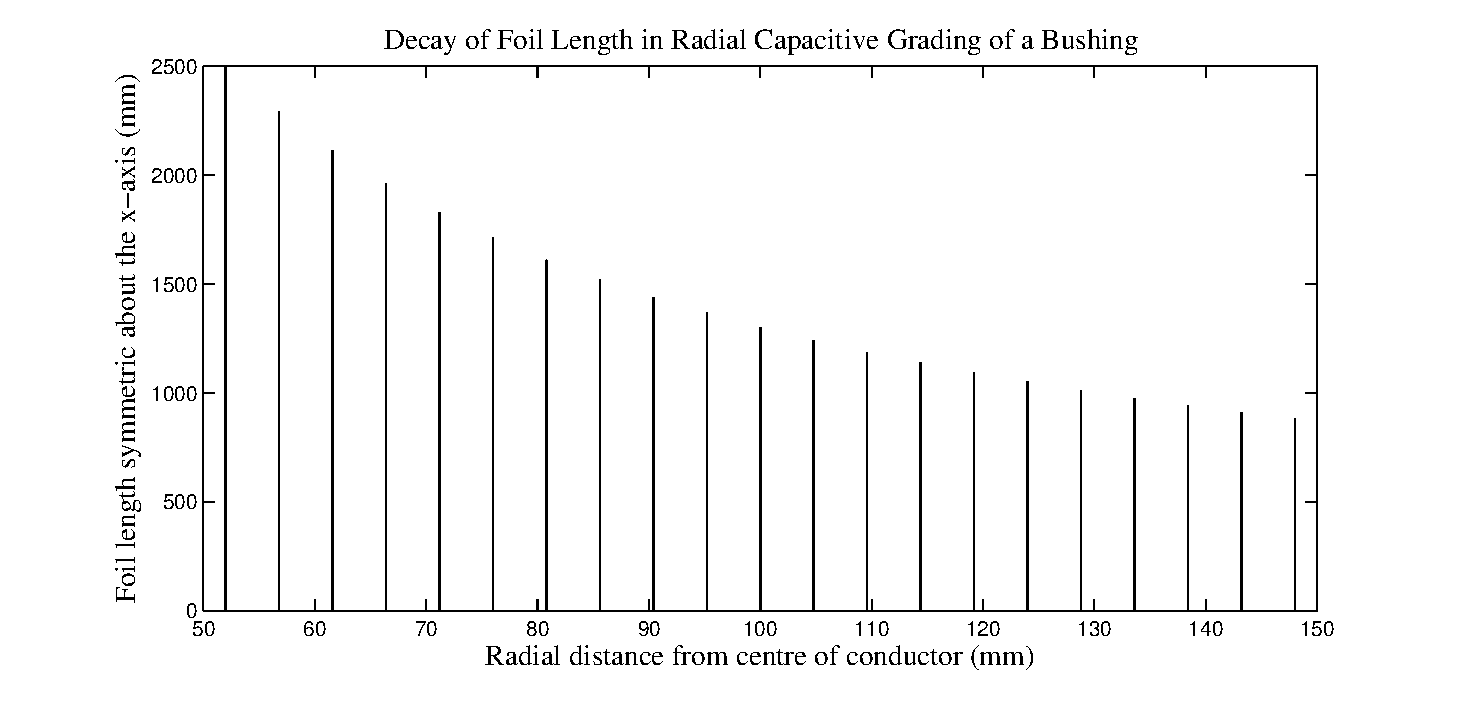
\includegraphics[height = 6cm]{../Matlab_Calculations/RadialGrade21ProfileWide.eps} 
	\label{Figure:21plot1}
  }
  \subfigure[Real Perspective]{
    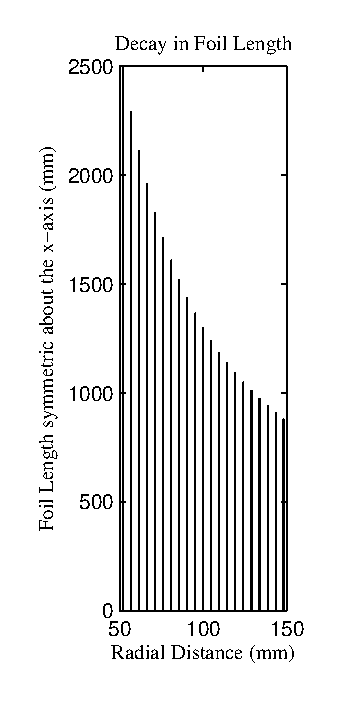
\includegraphics[height = 6cm]{../Matlab_Calculations/RadialGrade21ProfileSquash.eps} 
	\label{Figure:21plot2}
  }
\caption{Representation of foil radial position and length}
  \label{Figure:Both21plots}
\end{figure}

The final information required to be able to proceed to the simulation phase is the relative permittivity of each material.
This was gathered from \cite{Ahmed11} and is shown in table \ref{table:perm}.

\begin{table}[!htb]
\caption{Relative Permittivity of Materials}
\label{table:perm}
\begin{center}
\begin{tabular}{cc}
\toprule
\textbf{Material} & \textbf{Relative Permittivity ($\epsilon_r$)} \\ \toprule
Air & $1$ \\
Oil &$ 2.2$ \\
Paper Impregnated with Oil &$ 4$ \\
Aluminium & $10^8$\\
\bottomrule
\end{tabular}
\end{center}
\end{table}

